%%%%%%%%%%%%%%%%%%%% author.tex %%%%%%%%%%%%%%%%%%%%%%%%%%%%%%%%%%%
%
% sample root file for your "contribution" to a contributed volume
%
% Use this file as a template for your own input.
%
%%%%%%%%%%%%%%%% Springer %%%%%%%%%%%%%%%%%%%%%%%%%%%%%%%%%%


% RECOMMENDED %%%%%%%%%%%%%%%%%%%%%%%%%%%%%%%%%%%%%%%%%%%%%%%%%%%
\documentclass[graybox]{svmult}

% choose options for [] as required from the list
% in the Reference Guide

\usepackage{mathptmx}       % selects Times Roman as basic font
\usepackage{helvet}         % selects Helvetica as sans-serif font
\usepackage{courier}        % selects Courier as typewriter font
\usepackage{type1cm}        % activate if the above 3 fonts are
                            % not available on your system
%
\usepackage{makeidx}         % allows index generation
\usepackage{graphicx}        % standard LaTeX graphics tool
                             % when including figure files
\usepackage{multicol}        % used for the two-column index
\usepackage[bottom]{footmisc}% places footnotes at page bottom

\usepackage{qtree, bm, amsmath, amssymb, qtree, bm, multirow, textcmds, siunitx, mathrsfs, float, booktabs, color, soul}
\usepackage{natbib, setspace}
\usepackage[bb=boondox]{mathalfa}

\usepackage{tikz}
\definecolor{hfill_blue}{RGB}{208,229,249}
\definecolor{hfill_yellow}{RGB}{255,255,208}
\usetikzlibrary{trees,shapes}
\usetikzlibrary{matrix}
\tikzstyle{line} = [draw, thick]

% see the list of further useful packages
% in the Reference Guide

\makeindex             % used for the subject index
                       % please use the style svind.ist with
                       % your makeindex program

%%%%%%%%%%%%%%%%%%%%%%%%%%%%%%%%%%%%%%%%%%%%%%%%%%%%%%%%%%%%%%%%%%%%%%%%%%%%%%%%%%%%%%%%%
%\textsc{\textsc{\bibliographystyle{natbb}
%
%\bibliography{References_HTSF}

\def\ba{\begin{pmatrix}\tilde{\vec{b}}\\ \tilde{\vec{a}}\end{pmatrix}}
\def\GH{\begin{pmatrix}\vec{G}\\ \vec{F}\end{pmatrix}}
\def\Naive{Na\"{i}ve\ }
\def\naive{na\"{i}ve\ }



\begin{document}

\title*{Hierarchical Forecasting}
% Use \titlerunning{Short Title} for an abbreviated version of
% your contribution title if the original one is too long
\author{Name of First Author and Name of Second Author}
% Use \authorrunning{Short Title} for an abbreviated version of
% your contribution title if the original one is too long
\institute{Name of First Author \at Name, Address of Institute, \email{name@email.address}
\and Name of Second Author \at Name, Address of Institute \email{name@email.address}}
%
% Use the package "url.sty" to avoid
% problems with special characters
% used in your e-mail or web address
%
\maketitle

\abstract*{TBC}


\section{Introduction}

\textbf{Structure of the data with an macroeconomic example}\\

\textbf{Temporal hierarchies}\\

\textbf{Forecasting hierarchical time series}\\

\begin{itemize}
	\item Importance of coherency
	\item Point forecasting
	\item Probabilistic forecasting
\end{itemize}

\section{Hierarchical forecasting in macroeconomic data}

The key macroeconomic indicators such as Gross Domestic Product (GDP), inflation and monetary policies which are used to study the behavior and performance of an economy as a whole are it self aggregates of various other components.
For example, if we take the GDP growth, it is the aggregate of consumption, government expenditure, investments and net exports. These four components are again aggregates of some sub components. When we collect data for each of these individual variables over some time period, we will observe a collection of multiple time series that are bounded with some aggregation constraints. Thus the macroeconomic data are naturally forming cross sectional hierarchical time series.

If the interest is on a single macroeconomic variable along different time granularities, then it can be considered as a temporal hierarchy. For example, suppose we have monthly consumer product index (CPI) of a particular country. The quarterly CPI is then the aggregate of corresponding monthly CPI of each quarter. Similarly the yearly CPI is the aggregate of quarterly CPI of each year. Hence it will form a temporal hierarchy.

Macroeconomic forecasts are crucial for economic and business activities of any economy. Therefore this area of study has a long history in literature. Econometricians have developed various approaches for getting reliable economic forecasts using macroeconomic data. However, the information of aggregation structure in real data is limitedly used in literature. Moreover, having coherent forecasts will help the economists and policy makers for align decision making that impact for the whole economy. Therefore, our focus in this chapter is to introduce hierarchical forecasting methods for macroeconomic forecasting particularly for cross-sectional hierarchical data structures.

Obtaining coherent forecasts are independent from the forecasting models. That means forecasters were given the freedom to use any reliable forecasting method to obtain the forecasts for individual series in the hierarchy. Getting coherent forecasts is a post-processing technique which ensures the aggregation properties are preserved in the forecasts.   \\


\textcolor{red}{briefly discuss the point forecasts as well as probabilistic forecasts in the sense of macroeconomic data  }

\newpage
\section{Point forecasting}

Figure \ref{fig:simple tree} represents a simple two-level hierarchical structure. We use this example for simplicity in what follows. Denote as $y_{Tot,t}$ the value observed at time $t$ for the most aggregate (Total) series  corresponding to level 0 of the hierarchy. Below level 0, denote as $y_{i,t}$ the value of the series corresponding to node $i$, observed at time $t$. For example $y_{A,t}$ denotes the $t$th observation of the series corresponding to node A at level 1, $y_{AB,t}$ denotes the $t$th observation of the series corresponding to node AB at level 2, and so on.

\begin{figure}[!hbt]  \center
  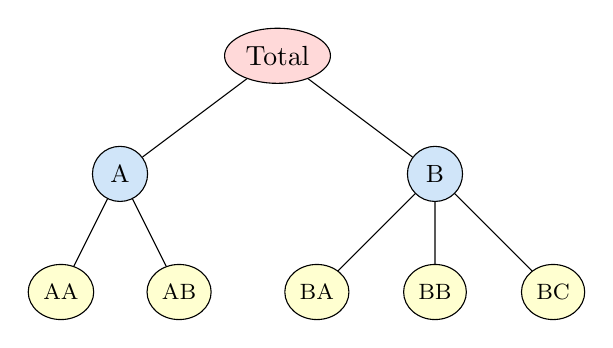
\begin{tikzpicture}
    \tikzstyle{every node}=[ellipse,draw,inner sep=2pt,minimum size=7mm,fill=red!15] %158,202,225
    \tikzstyle[level distance=.1cm]
    \tikzstyle[sibling distance=.1cm]
    %\tikzstyle{level 3}=[sibling distance=6.2mm,font=\tiny]
    \tikzstyle{level 1}=[sibling distance=40mm, font=\small, set style={{every node}+=[fill=hfill_blue]}]
    \tikzstyle{level 2}=[sibling distance=15mm, font=\footnotesize, set style={{every node}+=[fill=hfill_yellow]}]
    \node{Total}%[edge from parent fork down]
    child {node {A}
      child {node {AA}}
      child {node {AB}}
    }
    child {node {B}
      child {node {BA}}
      child {node {BB}}
      child {node {BC}}
    };
  \end{tikzpicture}
  \caption{A simple two-level hierarchical structure.}
  \label{fig:simple tree}
\end{figure}

\textcolor{red}{Need to say something about this. An alternative structure is grouped. In what follows we only use hierarchical reflecting also grouped unless there is a need to distinguish between them}.

\begin{figure}[!hbt]
\center
\tikzstyle{every node}=[inner sep=2pt,minimum size=7mm]
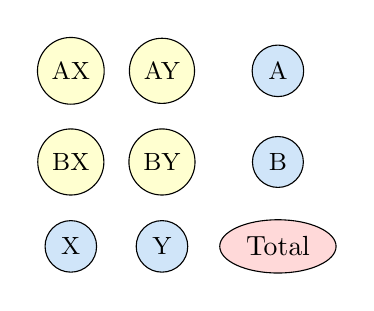
\begin{tikzpicture}
    \matrix[ampersand replacement=\&,column sep=0.3cm] {
        \node[circle,draw,fill=hfill_yellow, font=\small,distance=1cm] {AX};~ \&
        \node[circle,draw,fill=hfill_yellow,font=\small] {AY};~ \&
        \node[circle,draw,fill=hfill_blue, font=\small] {A}; \\[0.3cm]
        \node[circle,draw,fill=hfill_yellow, font=\small] {BX};~ \&
        \node[circle,draw,fill=hfill_yellow, font=\small] {BY};~ \&
        \node[circle,draw,fill=hfill_blue, font=\small] {B}; \\[0.3cm]
        \node[circle,draw,fill=hfill_blue, font=\small] {X};~ \&
        \node[circle,draw,fill=hfill_blue, font=\small] {Y};~ \&
        \node[ellipse,draw,fill=red!15] {Total}; \\
};
\end{tikzpicture}
  \caption{A simple two-level grouped structure.}
  \label{fig:simple grouped tree}
\end{figure}



Let $\vec{y}_t = (y_{Tot,t},y_{A,t}, y_{B,t},y_{AA,t}, y_{AB,t}, y_{BA,t}, y_{BB,t},y_{BC,t})'$, a vector containing observations across all series of the hierarchy at $t$. Similarly let $\vec{b}_t = (y_{AA,t}, y_{AB,t}, y_{BA,t}, y_{BB,t}, y_{BC,t})'$ a vector containing observations only for the bottom-level series. In general, $\vec{y}_t\in \mathbb{R}^n$ and $\vec{b}_t \in \mathbb{R}^m$ where $n$ denotes the number of total series in a hierarchy, $m$ the number of series at the bottom level, and $n>m$ always. In the simple example of Figure \ref{fig:simple tree}, $n=8$ and $m=5$.

Aggregation constraints dictate that $y_{Tot}=y_{A,t}+y_{B,t}=y_{AA,t}+y_{AB,t}+y_{BA,t}+y_{BB,t}+y_{BC,t}$,~ $y_{A,t}=y_{AA,t}+y_{AB,t}$ and $y_{B}=y_{BA,t}+y_{BB,t}+y_{BC,t}$. Hence we can write
\begin{equation}\label{eq:summing matrix}
\vec{y}_t = \vec{Sb}_t,
\end{equation}
where \begin{equation*}
\vec{S} = \begin{pmatrix}
1& 1& 1& 1 & 1 \\
1& 1& 0& 0 & 0\\
0& 0& 1& 1 & 1\\
& \multicolumn{3}{c}{\vec{I}_5} &
\end{pmatrix}
\end{equation*}
an $n\times m$ matrix referred to as the \textit{summing matrix} and $\vec{I}_m$ is an $m$-dimensional identity matrix. $\vec{S}$ reflects the linear aggregation constraints and in particular how the bottom-level series aggregate to levels above. Thus, columns of $\vec{S}$ span the linear subspace of $\mathbb{R}^n$ for which the aggregation constraints hold. We refer to this as the \textit{coherent subspace} and denote it by $\mathfrak{s}$. Notice that pre-multiplying a vector in $\mathbb{R}^m$ by $\vec{S}$ will result to an $n$-dimensional vector that lies in $\mathfrak{s}$.

\textcolor{red}{Add something to jump to coherent forecasts depending on the intro.}

\begin{definition}
A set of $h$-step ahead forecasts $\tilde{\vec{y}}_{t+h|t}$, stacked in the same order as $\vec{y}_{t}$ and generated using information up to and including time $t$,
are said to be coherent if $\tilde{\vec{y}}_{t+h|t} \in \mathfrak{s}$.
  \label{def:coherence}
\end{definition}

Hence a set of coherent forecasts respect the aggregation constraints across the hierarchy. That is the forecasts of lower level series aggregate up to their corresponding upper level series of the hierarchy and vice versa.
\\

\textcolor{red}{Do we need the following?}
Let us consider the smallest possible hierarchy with two bottom level series, $A$ and $B$ that add up to the top level $Tot$. Suppose $\breve{\vec{y}}_{t+h|t}$ of this hierarchy is given by $\breve{\vec{y}}_{t+h|t} = [\breve{y}_{Tot,t+h|t},\breve{y}_{A,t+h|t}, \breve{y}_{B,t+h|t}]$. Due to the aggregation structure we have $\breve{y}_{Tot,t+h|t}=\breve{y}_{A,t+h|t}+\breve{y}_{B,t+h|t}$. This implies that, even though  $\breve{\vec{y}}_{Tot,t+h|t} \in \mathbb{R}^3$, the points actually lie in $\mathfrak{s}\subset \mathbb{R}^3$, which is a two dimensional subspace within $\mathbb{R}^3$ space.

\textcolor{red}{I think the 3-series example talking about \textit{basis series} in the Prob Fore paper is useful here. Should we add?}


\subsection{Traditional forecasting approaches}
\textcolor{red}{Traditionally hierarchical structures were forecasted using these. We briefly present these here. For more details - give references.}

Traditional approaches involve selecting a level of aggregation, generating forecasts at the level and then linearly combining these to generate a set of coherent forecasts the rest of the structure.

\subsubsection{Bottom-up}
\textcolor{red}{Maybe we add these section headings here.}

In the \textit{bottom-up} approach, forecasts for the lowest level series are first generated. These are then aggregated to obtain forecasts for all the other levels of the hierarchy \citep{dunn1976}. In general this consists of first generating $\hat{\vec{b}}_{t+h|t} \in \mathbb{R}^m$, a set of $h$-step ahead forecasts for the bottom-level series. For the simple hierarchical structure of Figure \ref{fig:simple tree}, $\hat{\vec{b}}_{t+h|t} = (\hat{{y}}_{AA,t+h|t}, \hat{{y}}_{AB,t+h|t}, \hat{{y}}_{BA,t+h|t}, \hat{{y}}_{BB,t+h|t},\hat{{y}}_{BC,t+h|t}),$ where, $\hat{{y}}_{i,t+h|t}$ is the $h$-step ahead forecast of the series corresponding to node $i$. A set of coherent forecasts for the whole hierarchy is given by,
\begin{equation*}\label{eq:BU}
\tilde{\vec{y}}^{BU}_{t+h|t}=\vec{S\hat{\vec{b}}}_{t+h|t}.
\end{equation*}
Generating bottom-up forecasts has the advantage of no information being lost due to aggregation. However, bottom-level data can potentially be highly volatile or very noisy and therefore challenging to forecast.

\subsubsection{Top-down}

In contrast to bottom-up, \textit{top-down} approaches involve first generating forecasts for the most aggregated series and then disaggregating these down the hierarchy. In general, coherent forecasts generated from top-down approaches can be written as,

\begin{equation*}
\tilde{\vec{y}}^{TD}_{t+h|t}=\vec{S}\vec{p}\hat{y}_{Tot, t+h|t},
\end{equation*}
where $\vec{p} = (p_1,...,p_m)'$ is an $m$-dimensional vector consisting of a set of proportions which disaggregate the top-level forecast $\hat{y}_{Tot, t+h|t}$ to forecasts for the bottom-level series. These are then aggregated up by the summing matrix.

Two commonly used sets of proportions are:
\begin{equation*}
p_j = \frac{1}{T} \sum_{t=1}^{T}\frac{y_{j,t}}{y_{tot,t}},
\end{equation*}
for $j=1,\ldots,m$, where each $p_j$ reflects the average of the historical proportions of the bottom-level series $y_{j,t}$ over the period $t=1,\ldots,T$ relative to the total aggregate $y_{tot,t}$ and hence referred to as \textit{average historical proportions}, and
\begin{equation}
p_j = \frac{\frac{1}{T}\sum_{t=1}^{T}y_{j,t}}{\frac{1}{T}\sum_{t=1}^{T}y_{Tot,t}},
\end{equation}
where each proportion $p_j$ captures the average historical value of the bottom-level series $y_{j,t}$ relative to the average value of the total aggregate $y_{tot,t}$ and hence referred to as \textit{proportions of the historical averages}.

Both these approaches performed well in \cite{gross1990}. Their most convenient attribute is their simplicity. Generating a set of coherent forecasts involves only modelling and generating forecasts for the most aggregated top-level series. In general, such top-down approaches seem to produce quite reliable forecasts for the aggregate levels and they are useful with low count data. However, a significant disadvantage is the loss of information due to aggregation. Using such top-down approaches, is limited as does not allow to capture and model individual series characteristics such as time dynamics, special events, etc.

\textcolor{red}{Complete this if we decide to leave these in.}

To overcome this limitation, \cite{AthEtAl2009} introduced a new top-down approach which disaggregate the top level forecasts according to the proportions of forecasts rather than historical proportions. They found that their method outperforms the conventional top-down approach through an empirical application.

\textcolor{red}{This seems to be simply of combination of top and bottom level forecasts. We may drop it. }

Recently, \cite{Mircetic2017} proposed a modified approach to the conventional top-down methods, which involves forecasting $h$-step ahead proportions of bottom level series relative to the top level series. That is, let the ratio between the $j^\text{th}$ bottom level series and the top level series is given by, $p_{j,t}=y_{j,t}/y_{Tot,t}$, for $t=1,...,T$. Then this series of proportions will be forecast for the $h$-step ahead period, which is denoted by $\hat{p}_{j,T+h|T}$. These proportions will be then used as the disaggregate proportions to construct coherent top-down forecasts. Thus giving the elements of vector $\vec{p}$ as,

\begin{equation}
p_j = \hat{p}_{j,T+h|T}.
\end{equation}

This approach is much reliable, since it calculates the proportions as a function of time, rather than using the simple averages in traditional top-down methods.

\subsubsection{Middle-out}
\textcolor{red}{Add middle-out}

As shown by \cite{HynEtAl2011}, top-down methods are adding a bias component to each disaggregate level. Therefore, all these top-down approaches are producing biased forecasts even if the top level base forecasts are unbiased.

A compromise between these two approaches is the middle-out method which entails forecasting each series of a selected middle level in the hierarchy and then forecasting upper levels by the bottom-up method and lower levels by the top-down method.\\
Since this is a hybrid approach of bottom-up and top-down approaches it still remains the limitations of those two.

\subsection{Forecast reconciliation approaches}

A common theme of the traditional approaches discussed so far is that a single level of aggregation is first selected and then forecasts for that level are either aggregated-up, disaggregated-down or a combination of the two is used, in order to generate coherent forecasts for the whole hierarchy. Hence, these approaches are limited in only using information from a single level of aggregation and furthermore ignoring any correlations across levels.

An alternative framework that overcomes these limitations, first proposed by \citet{HynEtAl2011} and implemented by \citet{AthEtAl2009}, is one that involves forecast reconciliation. In a first step forecasts for all the series across all levels of the hierarchy are generated, ignoring the aggregation. We refer to these as \textit{base} forecasts and denote them as $\hat{\vec{y}}_{t+h|t}$. In general, base forecasts will not be coherent. An example of an exception is when a simple method such as a random walk is used to generate all base forecasts so that the coherent nature of the data is extended to the forecasts.

In a second step, base forecasts are revised and reconciled so that they become coherent. This is achieved by projecting the base forecasts $\hat{\vec{y}}_{t+h|t}$ onto the coherent subspace $\mathfrak{s}$, via a projection matrix $\vec{SG}$, resulting in a set of coherent forecasts $\tilde{\vec{y}}_{t+h|t}$. More specifically,
\begin{equation}\label{eq:recon}
\tilde{\vec{y}}_{t+h|t}=\vec{S}\vec{G}\hat{\vec{y}}_{t+h|t},
\end{equation}
where $\vec{G}$ is an $m\times n$ matrix that maps $\hat{\vec{y}}_{t+h|t}$ to the $\mathbb{R}^m$ space, producing a set of coherent forecasts for the bottom-level series, which are in turn mapped to the coherent subspace by the summing matrix $\vec{S}$ as defined in \eqref{eq:summing matrix}.

Note that all traditional approaches discussed so far can also be represented by \eqref{eq:recon} using an appropriately designed \vec{G}. For example, for the bottom-up approach, $\vec{G}=\begin{pmatrix}
\vec{0}_{(m \times n-m)} & \vec{I}_m
\end{pmatrix}$. We do not define these as reconciliation approaches as only forecasts from a single level of the hierarchy are used and subsequently these are either aggregated or disaggregated with no revision or reconciliation taking place.

\textcolor{red}{Revisit the following:}
It is worth discussing the unbiased property of these reconciled point forecasts.

Assume that the base forecasts are unbiased. That is, $E_{1:t}(\hat{\vec{y}}_{t+h|t})=\umu_{t+h|t}$ where $\umu_{t+h|t} = E_{1:t}[\vec{y}_{t+h}|\vec{y}_1,...,\vec{y}_t]$ is the true mean with the expectation taken over the observed sample up to time $t$. Then for any $\vec{G}$ such that $\vec{SGS}=\vec{S}$ or equivalently $\vec{SG}=\vec{I}_m$ the resulting coherent forecasts are also unbiased. \textcolor{red}{Can we tie in here this? Can we say: More generally \citep{Gamakumara2018} show that any $\vec{SG}$ that is a projection matrix will result to unbiased coherent forecasts}.

\subsubsection{OLS reconciliation}

\cite{HynEtAl2011} proposed to ``optimally'' reconcile the base forecasts through the following regression model:
\begin{equation}\label{eq:OLS}
\hat{\vec{y}}_{t+h|t} = \vec{S\ubeta}_{t+h|t} + \vec{\varepsilon}_{t+h|t},
\end{equation}
where $\vec{\ubeta}_{t+h|t}=E[\vec{b}_{t+h}|\vec{b}_1,.....,\vec{b}_t]$ is the unknown conditional mean of the bottom-level series and $\vec{\varepsilon}_{t+h|t}$ is the coherence or reconciliation error with mean zero and variance $\vec{V}$. The ordinary least squares (OLS) solution leads to the usual projection matrix $\vec{S}(\vec{S}'\vec{S})^{-1}\vec{S}'$, so that a set of coherent forecasts are obtained by,
\begin{equation*}
\tilde{\vec{y}}_{t+h|t}^{\text{OLS}} = \vec{S}(\vec{S}'\vec{S})^{-1}\vec{S}'\hat{\vec{y}}_{t+h|t}.
\end{equation*}
In this reconciliation, the incoherent forecasts are orthogonally projected to the coherent subspace $\mathfrak{s}$. Hence the OLS projection minimises the Euclidean distance between $\hat{\vec{y}}_{t+h|t}$ and $\tilde{\vec{y}}_{t+h|t}$.

\textcolor{red}{Can we add Tas's picture and talk about optimality in this sense.}

We should note that using the GLS solution in this context is not possible as \cite{WicEtAl2019} show that $\vec{V}$ is not identifiable.


\subsubsection{Optimal MinT reconciliation}

\cite{WicEtAl2019} build on the work of \citet{HynEtAl2011} on forecast reconciliation and introduce the MinT approach. MinT is optimal in the sense that given a set of unbiased base forecasts, MinT returns a set of best linear unbiased coherent forecasts using as $\vec{G}$ the unique solution that minimises the trace (hence MinT) of the variance of the forecast error of the coherent forecasts.

Let
\begin{equation}\label{eq:base errors}
\hat{\vec{e}}_{t+h|t} = \vec{y}_{t+h|t}-\hat{\vec{y}}_{t+h|t}
\end{equation}
denote the forecast errors for a set of unbiased base forecasts $\hat{\vec{y}}_{t+h|t}$, with Var$(\hat{\vec{e}}_{t+h|t})=\vec{W}_h$. Also let \begin{equation*}
\tilde{\vec{e}}_{t+h|t} = \vec{y}_{t+h|t}-\tilde{\vec{y}}_{t+h|t}
\end{equation*} denote a set of coherent forecast errors. Lemma 1 in \cite{WicEtAl2019} shows that for any matrix $\vec{G}$ such that $\vec{S}\vec{G}\vec{S}=\vec{S}$, $\text{Var}(\tilde{\vec{e}}_{t+h|t})=\vec{S}\vec{G}\vec{W}_h\vec{S}'\vec{G}'
$. Furthermore Theorem 1 shows that
\begin{equation} \label{eq:MinT}
\vec{G} = (\vec{S}'{\vec{W}}^{-1}_h\vec{S})^{-1}\vec{S}'{\vec{W}}^{-1}_h
\end{equation}
is the unique solution that minimises the tr$[\vec{S}\vec{G}\vec{W}_h\vec{S}'\vec{G}']$ subject to $\vec{S}\vec{G}\vec{S}=\vec{S}$. The unbiasedness constraint ensures that for a set of unbiased base forecasts the resulting reconciled forecasts are also unbiased. Note that unlike the GLS solution to \eqref{eq:OLS}, the MinT solution is a function of $\vec{W}_h$, the variance of the base forecast errors.

The MinT solution is an oblique projection of $\hat{\vec{y}}_{t+h|t}$ onto the coherent subspace $\mathfrak{s}$ and as shown by \cite{WicEtAl2019}, it minimises the Mahalonobis distance between $\hat{\vec{y}}_{t+h|t}$ and $\tilde{\vec{y}}_{t+h|t}$.

A significant advantage of the MinT reconciliation solution is that it is the first to incorporate the full correlation structure of the hierarchy via ${\vec{W}}_{h}$. However, estimating ${\vec{W}}_{h}$ is challenging, especially for $h>1$. Of course setting ${\vec{W}}_{h}=k_h\vec{I}_n$ for all $h$ where $k_h>0$ is a proportionality constant, leads to the OLS solution of \cite{HynEtAl2011}. A disadvantage of this simplifying solution, further to not accounting for the correlations across series, is that the homoscedastic diagonal does not account for the scale differences between the levels of the hierarchy due to aggregation. \textcolor{red}{However OLS does well in practice because as discussed it minimises the Euclidean distance and blah blah. Not sure how much we want to say here.}

\citet{WicEtAl2019} present possible alternative estimators for ${\vec{W}}_{h}$ and show that these lead to different $\vec{G}$ matrices. We summarise these below.

\begin{itemize}
    \item Set ${\vec{W}}_{h}=\text{diag}(\hat{\vec{W}}_{1})$ for all $h$, where $k_{h} > 0$ and
        $$
        \hat{\vec{W}}_{1} = \frac{1}{t}\sum_{k=1}^{t} \hat{\vec{e}}_{k}\hat{\vec{e}}_{k}'
        $$
        is the unbiased sample estimator of the in-sample one-step-ahead base forecast errors as defined in~\eqref{eq:base errors}. This estimator scales the base forecasts using the variance of the in-sample residuals and is therefore describes and referred to as a WLS estimator.
    \item  Set $\vec{W}_{h}=k_{h}\hat{\vec{W}}_{1}$, for all $h$, where $k_{h} > 0$, the unrestricted sample covariance estimator for $h=1$. Although this is relatively simple to obtain and provides a good solution for small hierarchies, it does not provide reliable results a $m$ grows compared to $t$. We refer to this a the MinT(Sample) estimator.
    \item Set $\vec{W}_{h}=k_{h}\hat{\vec{W}}_{1}^D$, for all $h$, where $k_{h} > 0$, $\hat{\vec{W}}^{D}_{1} = \lambda_{D} \text{diag}(\hat{\vec{W}}_{1}) + (1 - \lambda_{D})\hat{\vec{W}}_{1}$ is a shrinkage estimator with diagonal target, and shrinkage intensity parameter

        $$\hat{\lambda}_{D} = \frac{\sum_{i \ne j}\hat{Var}(\hat{r}_{ij})}{\sum_{i \ne j}\hat{r}_{ij}^2},$$

        %$$\hat{\lambda}_{D} = \frac{\sum_{i \neq j} \widehat{\var(\hat{r}_{ij})}} {\sum_{i \neq j} \hat{r}_{ij}^{2}},$$

        where $\hat{r}_{ij}$ is the $ij$th element of $\hat{\bm{R}}_{1}$, the $1$-step-ahead sample correlation matrix as proposed by \citet{Schafer2005}. Hence, off-diagonal elements of $\hat{\vec{W}}_1$ are shrunk towards zero while diagonal elements (variances) remain unchanged. We refer to this as the MinT(Shrink) estimator.
\end{itemize}

\section{Hierarchical probabilistic forecasting}

Point forecasts are limited because they provide no indication of forecast uncertainty. Providing prediction intervals helps \citep{Shang2017a}, but a richer description of forecast uncertainty is obtained by estimating the entire forecast distribution. These are often called ``probabilistic forecasts'' \citep{Gneiting2014}. For example, \citet{McSharry2005} produced probabilistic forecasts for electricity demand, \citet{BenTaieb2017} for smart meter data, \citet{Pinson2009} for wind power generation, and \citet{Gel2004}, \citet{Gneiting2005a} and \citet{Gneiting2005} for various weather variables.

Even though the point forecasts in hierarchical time series is well studied and having an established literature, the hierarchical probabilistic forecasting is still an emerging area of interest. There's is only a few studies in published literature. The uncertainly around $\vec{y}_{t+h|t}$ is referred to as the probabilistic forecasts in hierarchical time series. Due to the aggregation nature of the data, these should also lie in the coherent subspace $\mathfrak{s}$. If so, we call them as coherent probabilistic forecasts.

\cite{Taieb2017} defined the coherent probabilistic forecasts in terms of convolution. That is, the predictive distributions of a hierarchy is said to be coherent, if the convolution of forecast distributions of disaggregate series is equal to the forecast distribution of the corresponding aggregate series. Based on this, they proposed an algorithm to produce coherent probabilistic forecasts and applied it to UK electricity smart meter data.

Analogous to point forecast reconciliation, we can reconcile the forecast distributions to get coherent probabilistic forecasts. This will start with an incoherent forecast distribution of the whole hierarchy which was obtained by gathering all information available, and then projecting that to the coherent subspace similar in the point forecasting case. Geometric intuition behind the probabilistic forecast reconciliation is discussed in \cite{Gamakumara2018}.

\subsection{Probabilistic forecast reconciliation in the Gaussian framework}

Suppose we have a set of hierarchical time series where each realisation follows a multivariate Guassian distribution. i.e., $\vec{y}_T \sim \mathscr{N}(\vec{\mu}_T, \Sigma_T)$ where both $\vec{\mu}_T$ and $\Sigma_T$ lives in the coherent subspace $\mathfrak{s}$ due to the aggregation structure of the hierarchy. We are interested in estimating the predictive Gaussian distribution of $\vec{Y}_{T+h}| \vec{\mathscr{I}}_T$ where $\vec{\mathscr{I}}_T= \{\vec{y}_1,\vec{y}_2,\dots.,\vec{y}_T\}$, which should also lives in $\mathfrak{s}$. Since Gaussian distributions are uniquely characterised by the first two moments, it is sufficient to have the mean and variance forecasts to get the Gaussian predictive distributions of the hierarchy.

Assume we have fit the time series models for each series of the hierarchy by considering all the available information. Using these fitted models we can estimate the means and variance forecasts of the hierarchy which are denoted by $\vec{\hat{\mu}}_{T+h}$ and $\hat{\Sigma}_{T+h}$ respectively. Each element in $\vec{\hat{\mu}}_{T+h}$ corresponds to the mean forecast of each series in the hierarchy and these elements are stacked in the same order as $\vec{y}_t$. Similarly $\hat{\Sigma}_{T+h}$ contains variances and covariances of all series in the hierarchy. One can either fit univariate models for each individual series of the hierarchy or fit multivariate models by considering the correlation structure of the series for getting these forecasts. However as long as the aggregation structure is not imposed, it is very unlikely that these forecasts will be coherent. Thus it comes to the point of reconciliation.

Reconciling Gaussian forecast distribution is all about reconciling the incoherent means and variance of forecasts. That is, the reconciled Gaussian distribution is given by $\mathscr{N}(\vec{\tilde{\mu}}_{T+h}, \tilde{\Sigma}_{T+h})$, where,

\begin{equation}\label{eq:17}
\vec{\tilde{\mu}}_{T+h} = \vec{SG}\vec{\hat{\mu}}_{T+h},
\end{equation}
and
\begin{equation}\label{eq:18}
\tilde{\Sigma}_{T+h} = \vec{SG}\hat{\Sigma}_{T+h}\vec{G'S'}.
\end{equation}

A more rigorous explanation about deriving these equations can be found in \cite{Gamakumara2018}. Depending on the choice of $\vec{G}$ we will get different Gaussian forecast distributions. The same choices of $\vec{G}$ matrices that has been used in the point forecasting case can be used in reconciling Gaussian forecast distributions. It is also worth mentioning that, due to the aggregation constraints, the distributions lies in $\mathfrak{s}$, which is a lower dimensional subspace of $\mathbb{R}^n$. Therefore, these reconciled Gaussian distributions are degenerate.


\subsection{Probabilistic forecast reconciliation in the non-parametric framework}

In many applications it may not reasonable to assume parametric forecasting distributions. Therefore, non-parametric approaches has been widely used for probabilistic forecasts in different disciplines. For example, ensemble forecasting in weather applications (\cite{Gneiting2005}, \cite{Gneiting2014}, \cite{Gneiting2008}), bootstrap based approaches (\cite{Manzan2008}, \cite{Vilar2013}).

Non-parametric approaches are also important in hierarchical forecasting as in most applications they have millions of time series which are often difficult to assume parametric distributions. Further, for data with heavy tails, it is often misleading to assume Gaussianity. The algorithm introduced by \cite{Taieb2017} is also a non-parametric approach as it does not make any distributional assumptions. They first generate, a sample from the bottom level predictive distribution, and then aggregate to obtain coherent probabilistic forecasts of the upper levels of the hierarchy. Initially they use MinT algorithm to reconcile the means of the bottom level forecast distributions, and then a copula-based approach is employed to model the dependency structure of the hierarchy. Resulting multi-dimensional distribution is used to generate the empirical forecast distributions for all bottom-level series which are then aggregated to obtain the empirical forecast distribution for the entire hierarchy. Although the means of forecast distributions are reconciled, the predictive distributions were obtained through a bottom-up based approach. Therefore this approach is not a reconciliation method as it does not use all the information from the hierarchy when producing coherent probabilistic forecasts.

\cite{Jeon2018} is the only existing study that does reconciliation in probabilistic hierarchical forecasts. This method is based on cross-validation and it also does not assume any parametric distributions for predictive densities. However they applied this method particularly for temporal hierarchies.

\cite{Gamakumara2018} discussed that reconciling the draws from incoherent forecast distribution will give draws from a reconciled forecast distribution. Employing this fact, we introduce a novel method based on a bootstrap approach. This involves a two steps process. In the first step we obtain possible sample paths from the incoherent forecast distributions. This follows by the reconciliation step which projects each sample path to the coherent subspace. These steps will be discussed in detail below.

\subsection*{Step 1: Obtaining incoherent probabilistic forecasts}

Suppose we fit univariate time series models for the series at each node in the hierarchy, by using past observations up to time $T$. Using these fitted models, we can generate $h$ step ahead future sample paths for each node, by conditioning on past observations. In order to capture the dependency structure of the hierarchy, we incorporate bootstrapped training errors from the fitted models. That is, let $\varGamma_{(T \times n)}=(\vec{e}_1,\vec{e}_2,.....,\vec{e}_T)'$ denote the in-sample residual matrix where, $\vec{e}_t=\vec{y}_t-\hat{\vec{y}}_t$ is a vector that consists of residuals in each node at time $t$ and stacked in the same order as $\vec{y}_t$. $\varGamma$ is also referred to as the matrix of in-sample errors. Then we block bootstrap a sample of size $h$ from $\varGamma$, and these bootstrapped errors will be incorporated as the error series for simulating future paths. Taking block bootstrapped in-sample errors in generating future paths will implicitly model the dependency structure of the hierarchy. These simulated future sample paths will be then formed in a vector $\hat{\vec{y}}_{T+h|T}^b$ by stacking the sample paths of each node in the same order as $\vec{y}_t$. As such we generate a sample of $N$ future paths for the hierarchy. We can denote this sample by a $(N \times n)$ matrix $\hat{\vec{Y}}^b_{T+h|T}$ where,

\begin{equation} \label{eq:19}
\hat{\vec{Y}}^b_{T+h|T}=\begin{pmatrix}
\hat{\vec{y}}_{1,T+h|T}^b\\
\hat{\vec{y}}_{2,T+h|T}^b\\
\vdots\\
\hat{\vec{y}}_{N,T+h|T}^b
\end{pmatrix}.
\end{equation}

Although the dependency structure of the hierarchy is captured through the bootstrap in-sample errors, the aggregation structure will not be reflected through these sample paths. Therefore, these future paths are incoherent and thus considered as a possible sample from the incoherent probabilistic forecast distribution of the hierarchy.

\subsection*{Step 2: Reconciling future sample paths}

The second step is to project these sample paths to the coherent subspace. Then we get a set of reconciled future paths which form a possible sample from the reconciled probabilistic forecast distribution. Similar to the projection used in the point forecast reconciliation, we project each sample path through the projection $\vec{SG}$. Then we get,

\begin{equation} \label{eq:20}
\tilde{\vec{y}}_{i,T+h}^b = \vec{SG}\hat{\vec{y}}_{i,T+h}^b, \quad i = 1, ..., N
\end{equation}
and let
\begin{equation}\label{eq:21}
\tilde{\vec{Y}}^b_{T+h|T}=\begin{pmatrix}
\tilde{\vec{y}}_{1,T+h|T}^b\\
\tilde{\vec{y}}_{2,T+h|T}^b\\
\vdots\\
\tilde{\vec{y}}_{N,T+h|T}^b
\end{pmatrix}
\end{equation}
where, $\tilde{\vec{y}}_{i,T+h}^b \in \mathfrak{s}$ denote a $h$-step-ahead reconciled future paths for $i=1,...,N$. $\tilde{\vec{Y}}^b_{T+h|T}$ form an empirical coherent forecast distribution of the hierarchy that lies in the coherent subspace $\mathfrak{s}$. As we discussed in point forecast reconciliation methods, different estimates of $\vec{G}$ provide alternative estimates of reconciled future paths. We can also obtain bottom-up based future paths by simply aggregating the future paths of bottom level series for their respective upper levels. This is referred to as bottom-up future paths. Even though the bottom-up approach generates coherent probabilistic forecasts, it cannot be considered as a reconciliation method since it use only half of the information.


\section{Evaluation}

In this section we briefly discuss the methods that we use to measure the forecast accuracy of hierarchical forecasts.

\subsection{Point forecast evaluation}

Any existing point forecast evaluation method can be used to evaluate the accuracy of hierarchical point forecast. We are mainly using Mean Squared Error (MSE) and Mean Absolute Scaled Error (MASE) in our empirical application. Mathematical expression for these measures are given below.

\begin{equation}\label{eq:22}
MSE = mean(e^2_{t+h}),
\end{equation}
and
\begin{equation}\label{eq:23}
 MASE = mean(q_{t+h}),
\end{equation}
where $q_{t+h} = \frac{e_{t+h}}{\frac{1}{T-m}\sum_{j=m+1}^{T}|y_j - y_{j-m}|}$. Further $e_{t+h}$ is the forecast error, which is the difference between forecast and realisation.

MSE is a scaled dependent measure. Therefore to compare series in different scales or with different units, MASE is preferred. For more details on different point forecast accuracy measures refer to \cite{hyndman2018forecasting}.

\subsection{Probabilistic forecast evaluation}

Forecast accuracy of probabilistic forecasts can be evaluated using scoring rules \cite{Gneiting2014}. Scoring rules provides a summary measurement based on the relationship between realisation and the forecast distribution. However, not all scoring rules are applicable for hierarchical probabilistic forecast evaluation. An comprehensive discussion on this can be found in \cite{Gamakumara2018}.

Since the whole forecast distribution of the hierarchy is a multivariate distribution, the forecast accuracy should also be assessed in the multivariate framework. Therefore using multivariate scoring rules is helpful. Energy score \citep{Gneiting2008} and variogram scores \citep{SCHEUERER2015} are the mainly using multivariate scoring rules in hierarchical framework. Further, multivariate log score \citep{Gneiting2007} can also be used for evaluating parametric forecast distributions. The mathematical expressions for these are given table \ref{table:scoringrules}.

\begin{table}[!b]
	\caption{Scoring rules to evaluate multivariate forecast densities. $\breve{\vec{y}}_{T+h}$ and $\breve{\vec{y}}^*_{T+h}$ be two independent random vectors from the coherent forecast distribution $\breve{\vec{F}}$ with the density function $\breve{\vec{f}}(\cdot)$ at time $T+h$ and $\vec{y}_{T+h}$ is the vector of realizations. Further $\breve{Y}_{T+h,i}$ and $\breve{Y}_{T+h,j}$ are $i$th and $j$th components of the vector $\breve{\vec{Y}}_{T+h}$. Moreover, the variogram score is given for order $p$ where, $w_{ij}$ are non-negative weights.}\label{table:scoringrules}
	\centering\small\setstretch{1.3}
	\begin{tabular}{@{}lp{8.1cm}}
		\toprule
		\textbf{Scoring rule}  & \textbf{Expression}           \\
		\midrule
		\text{Log score}       &
		$\text{LS}(\breve{\bm{F}},\bm{y}_{T+h}) = -\log {\breve{\bm{f}}(\bm{y}_{T+h})}$ \\\\[-0.2cm]
		\text{Energy score}    &
		$\text{eS}(\breve{\bm{Y}}_{T+h},\bm{y}_{T+h}) =
		E_{\breve{\bm{F}}}
		\|\breve{\bm{Y}}_{T+h}-\bm{y}_{T+h}\|^\alpha -$ \par\hfill
		$\frac{1}{2}E_{\breve{\bm{F}}}\|\breve{\bm{Y}}_{T+h}-\breve{\bm{Y}}^*_{T+h}\|^\alpha$, \,\, $\alpha \in (0,2]$ \\\\[-0.2cm]
		\text{Variogram score} &
		$\text{VS}(\breve{\bm{F}}, \bm{y}_{T+h}) =
		\sum\limits_{i=1}^{n}
		\sum\limits_{j=1}^{n}
		w_{ij}\Big(|y_{T+h,i} - y_{T+h,j}|^p -$ \par\hfill
		$E_{\breve{\bm{F}}}|\breve{Y}_{T+h,i}-\breve{Y}_{T+h,j}|^p\Big)^2$ \\
		\bottomrule
	\end{tabular}
\end{table}

Log score is easy to use if the parametric forecast distributions are available. However, \cite{Gamakumara2018} showed that the multivariate log scores are inappropriate for the comparisons between incoherent and coherent forecast distributions. This is due to the degeneracy of multivariate coherent forecast distributions.

Energy score and variogram score can be used in any comparisons between multivariate hierarchical forecast distributions. The expectations in these scoring rules can be approximated by the sample means of simulated samples.

It would be also interested to see the performance of forecast distributions of individual series in the hierarchy. To measure these we use univariate scoring rules such as Continuous Rank Probability Score (CRPS) and univariate log score \citep{Gneiting2008}. The mathematical expression for CRPS is given by,

\begin{equation} \label{eq:24}
\text{CRPS}(\breve{F}_i,y_{T+h,i}) = E_{\breve{F}_i}|\breve{Y}_{T+h,i}-y_{T+h,i}| - \frac{1}{2}E_{\breve{F}_i}|\breve{Y}_{T+h,i}-\breve{Y}^*_{T+h,i}|,
\end{equation}
where $\breve{Y}_{T+h,i}$ and $\breve{Y}^*_{T+h,i}$ are two independent copies from the $i$th reconciled marginal forecast distribution $\tilde{F}_i$ of the hierarchy and $y_{T+h,i}$ is the $i$th realization from the true marginal distribution $G_i$. As in multivariate scoring rules, the expectations can be approximated by the sample average.

\subsection{Comparison between different forecasting methods}

We are mainly interested to evaluate the hierarchical forecasts in two aspects. One is to examine whether the having coherent forecasts is improving the forecast accuracy. This can be evaluated by comparing the incoherent forecasts with any coherent forecasts in both point as well as probabilistic framework. Secondly we are interested in finding the best reconciliation method by comparing reconciled forecast from different reconciliation methods.

For any comparison we use Skill score as defined in \citep{Gneiting2007}. For a given forecasting method, evaluated by a particular scoring rule $S(\cdot)$ , the skill score can be calculated as follows,
\begin{equation} \label{eq:25}
Ss[S_B(\cdot)] = \frac{S_B(\bm{Y},\bm{y})^{\text{ref}} - S_B(\breve{\bm{Y}},\bm{y})}{S_B(\bm{Y},\bm{y})^{\text{ref}}}\times 100\%,
\end{equation}
where $S_B(\cdot)$ is average score over $B$ replicates and $S_B(\bm{Y},\bm{y})^{\text{ref}}$ is the average score of the reference forecasting methods. Thus $Ss[S_B(\cdot)]$ gives the percentage improvement of the preferred forecasting method relative to the reference method. Any positive value indicates that method is superior to the reference method, whereas any negative value of $Ss[S_B(\cdot)]$ indicate that the method we compared is poor than the reference method.

\section{Empirical study}

\begin{itemize}
	\item GDP of Australia
	\item []
	\item How GDP is measured
		\begin{itemize}
			\item Production, Income and Expenditure approach
			\item Explain the hierarchy
		\end{itemize}
	\item Issues with data
		\begin{itemize}
			\item Why use current price rather than constant price (This is why we ignores production approach)
			\item What is statistical discrepancy
			\item Frequency of data
			\item Does the data satisfies coherency
		\end{itemize}
	
	\item Forecasting methods
		\begin{itemize}
			\item Add a figure of all time series in income approach.
			Explain why traditional methods might not work using these time series as forecasting one layer of the hierarchy will ignore the structural information of individual time series to be used in the forecasts.
			
			\item Explain ETS and ARIMA forecasting methods briefly
			\item Hierarchical forecasting
		\end{itemize}
\end{itemize}


\subsection{Point forecasting}

\subsubsection{Income approach}


\begin{table}[H]
	\caption{Summary of point forecast in income approach}
	\centering
	\resizebox{\linewidth}{!}{
		\begin{tabular}{@{}lSSSSSSSSSSSSSSSS@{}}
			\toprule
			\multicolumn{1}{c}{ } & \multicolumn{8}{c}{ETS} & \multicolumn{8}{c}{ARIMA} \\
			\cmidrule(lr){2-9} \cmidrule(l){10-17}
			\multicolumn{1}{c}{ } & \multicolumn{4}{c}{MSE} & \multicolumn{4}{c}{MASE} & \multicolumn{4}{c}{MSE} & \multicolumn{4}{c}{MASE} \\
			\cmidrule(lr){2-5} \cmidrule(lr){6-9} \cmidrule(lr){10-13} \cmidrule(l){14-17}
			Method & h=1 & h=2 & h=3 & h=4 & h=1 & h=2 & h=3 & h=4 & h=1 & h=2 & h=3 & h=4 & h=1 & h=2 & h=3 & h=4\\
			\midrule
			&&&&&&&\multicolumn{3}{c}{Most aggregate level}&&&&&&&\\
			\midrule
			Benchmark & -418.74 & -135.45 & -36.30 & -3.10 & -127.28 & -69.39 & -28.70 & -21.03 & -420.06 & -128.25 & -39.11 & -15.49 & -140.89 & -67.24 & -38.84 & -28.69\\
			
			Base & 0.00 & 0.00 & 0.00 & 0.00 & 0.00 & 0.00 & 0.00 & 0.00 & 0.00 & 0.00 & 0.00 & 0.00 & 0.00 & 0.00 & 0.00 & 0.00\\
			
			Bottom-up & -17.93 & -3.68 & 7.80 & 9.35 & -5.62 & -3.49 & -4.36 & -15.49 & -9.15 & 7.01 & 10.74 & 13.18 & -13.13 & -1.12 & -6.25 & -9.78\\
			
			OLS & -0.18 & 3.45 & 6.05 & 6.70 & 0.05 & 0.96 & 3.47 & 1.50 & 2.12 & 2.46 & 2.54 & 1.92 & -0.83 & 1.84 & 0.75 & 0.62\\
			
			WLS & -4.05 & 5.59 & 11.57 & 13.09 & -0.67 & 2.96 & 3.32 & -2.27 & 2.41 & 6.80 & 9.35 & 9.71 & -4.14 & 1.41 & 1.05 & -1.78\\
			
			MinT Shrink & -0.72 & 5.86 & 9.33 & 9.70 & 3.25 & 5.14 & 4.63 & -1.15 & 7.06 & 9.05 & 8.63 & 9.73 & -0.14 & 0.93 & 1.23 & 0.39\\
			\midrule
			&&&&&&\multicolumn{5}{c}{Average across all aggregate levels}&&&&&&\\
			\midrule
			Benchmark & -320.17 & -101.63 & -29.68 & -2.32 & -96 & -40.28 & -11.83 & -1.92 & -298.21 & -86.44 & -19.78 & 0.71 & -78.18 & -36.49 & -11.83 & -2.91\\
			
			Base & 0.00 & 0.00 & 0.00 & 0.00 & 0 & 0.00 & 0.00 & 0.00 & 0.00 & 0.00 & 0.00 & 0.00 & 0.00 & 0.00 & 0.00 & 0.00\\
			
			Bottom-up & -7.64 & -2.49 & 0.73 & 1.55 & -2 & 0.00 & -2.15 & -1.92 & 1.61 & 8.32 & 5.18 & 9.05 & 1.82 & 1.35 & -1.08 & 0.00\\
			
			OLS & 3.16 & 3.29 & 2.91 & 2.92 & 2 & 2.78 & 2.15 & 1.92 & 4.79 & 4.33 & 3.05 & 3.37 & 1.82 & 1.35 & 1.08 & 1.94\\
			
			WLS & 3.61 & 4.84 & 4.39 & 4.45 & 4 & 4.17 & 2.15 & 1.92 & 7.89 & 8.49 & 6.94 & 8.15 & 3.64 & 2.70 & 1.08 & 1.94\\
			
			MinT Shrink & 6.46 & 5.18 & 2.39 & 1.54 & 6 & 4.17 & 3.23 & 2.88 & 12.69 & 11.96 & 6.76 & 8.69 & 7.27 & 5.41 & 2.15 & 4.85\\
			\midrule
			&&&&&&\multicolumn{5}{c}{Average across bottom level}&&&&&&\\
			\midrule
			Benchmark & -200.06 & -71.72 & -21.93 & -0.40 & -61.02 & -30.67 & -11.11 & -2.02 & -191.76 & -64.02 & -7.71 & 6.65 & -63.79 & -32.43 & -13.64 & -4.12\\
			
			Base & 0.00 & 0.00 & 0.00 & 0.00 & 0.00 & 0.00 & 0.00 & 0.00 & 0.00 & 0.00 & 0.00 & 0.00 & 0.00 & 0.00 & 0.00 & 0.00\\
			
			Bottom-up & 0.00 & 0.00 & 0.00 & 0.00 & 0.00 & 0.00 & 0.00 & 0.00 & 0.00 & 0.00 & 0.00 & 0.00 & 0.00 & 0.00 & 0.00 & 0.00\\
			
			OLS & 0.66 & -2.57 & -3.50 & -3.73 & -23.73 & -26.67 & -18.89 & -12.12 & -2.88 & -5.33 & -2.55 & -4.91 & -20.69 & -24.32 & -22.73 & -20.62\\
			
			WLS & 6.18 & 3.62 & 1.38 & 0.28 & 1.69 & 0.00 & -1.11 & 0.00 & 2.43 & -0.25 & 2.93 & 0.29 & 0.00 & -1.35 & -1.14 & 0.00\\
			
			MinT Shrink & 8.78 & 4.34 & 0.58 & -1.43 & 3.39 & 1.33 & 1.11 & 1.01 & 4.81 & 1.57 & 2.15 & 0.47 & 0.00 & -1.35 & -1.14 & 0.00\\
			\midrule
			&&&&&&\multicolumn{5}{c}{Average across all levels}&&&&&&\\
			\midrule
			Benchmark & -295.40 & -96.29 & -28.41 & -2.01 & -71.43 & -33.78 & -10.99 & -1.98 & -276.70 & -82.54 & -17.73 & 1.68 & -68.42 & -33.78 & -12.22 & -4.04\\
			
			Base & 0.00 & 0.00 & 0.00 & 0.00 & 0.00 & 0.00 & 0.00 & 0.00 & 0.00 & 0.00 & 0.00 & 0.00 & 0.00 & 0.00 & 0.00 & 0.00\\
			
			Bottom-up & -6.06 & -2.05 & 0.61 & 1.31 & 0.00 & 0.00 & -1.10 & 0.00 & 1.28 & 6.88 & 4.30 & 7.57 & 1.75 & 0.00 & 0.00 & 0.00\\
			
			OLS & 2.64 & 2.24 & 1.86 & 1.87 & -14.29 & -14.86 & -10.99 & -6.93 & 3.24 & 2.65 & 2.09 & 2.01 & -12.28 & -14.86 & -13.33 & -12.12\\
			
			WLS & 4.14 & 4.62 & 3.89 & 3.79 & 3.57 & 1.35 & 0.00 & 0.99 & 6.79 & 6.97 & 6.25 & 6.86 & 1.75 & 0.00 & 0.00 & 1.01\\
			
			MinT Shrink & 6.94 & 5.03 & 2.09 & 1.07 & 5.36 & 2.70 & 2.20 & 1.98 & 11.10 & 10.15 & 5.98 & 7.34 & 3.51 & 1.35 & 0.00 & 1.01\\
			\bottomrule
		\end{tabular}
	}
\end{table}

\subsubsection{Expenditure approach}

\begin{table}[H]
	\caption{Summary of point forecast in expenditure approach}
	\centering
	\resizebox{\linewidth}{!}{
		\begin{tabular}{@{}lSSSSSSSSSSSSSSSS@{}}
			\toprule
			\multicolumn{1}{c}{ } & \multicolumn{8}{c}{ETS} & \multicolumn{8}{c}{ARIMA} \\
			\cmidrule(lr){2-9} \cmidrule(l){10-17}
			\multicolumn{1}{c}{ } & \multicolumn{4}{c}{MSE} & \multicolumn{4}{c}{MASE} & \multicolumn{4}{c}{MSE} & \multicolumn{4}{c}{MASE} \\
			\cmidrule(lr){2-5} \cmidrule(lr){6-9} \cmidrule(lr){10-13} \cmidrule(l){14-17}
			Method & h=1 & h=2 & h=3 & h=4 & h=1 & h=2 & h=3 & h=4 & h=1 & h=2 & h=3 & h=4 & h=1 & h=2 & h=3 & h=4\\
			\midrule
			&&&&&&&\multicolumn{3}{c}{Most aggregate level}&&&&&&&\\
			\midrule
			Benchmark & -418.74 & -135.45 & -36.30 & -3.10 & -127.28 & -69.39 & -28.70 & -21.03 & -420.06 & -128.25 & -39.11 & -15.49 & -140.89 & -67.24 & -38.84 & -28.69\\
			
			Base & 0.00 & 0.00 & 0.00 & 0.00 & 0.00 & 0.00 & 0.00 & 0.00 & 0.00 & 0.00 & 0.00 & 0.00 & 0.00 & 0.00 & 0.00 & 0.00\\
			
			Bottom-up & -24.62 & -6.94 & 13.89 & 19.17 & -6.68 & -2.54 & 3.99 & -2.73 & -44.70 & -16.08 & 0.96 & 7.78 & -18.84 & -1.99 & -6.89 & -8.10\\
			
			OLS & 8.32 & 8.19 & 11.30 & 11.18 & 6.06 & 5.67 & 6.74 & 4.30 & 5.37 & 5.72 & 7.59 & 7.70 & 0.43 & 3.56 & 3.38 & 4.25\\
			
			WLS & 8.75 & 10.69 & 17.96 & 18.90 & 8.48 & 7.91 & 9.37 & 4.83 & 0.97 & 5.08 & 10.24 & 11.50 & 0.15 & 2.91 & 2.11 & 3.12\\
			
			MinT Shrink & 9.80 & 10.20 & 16.71 & 18.44 & 9.02 & 6.77 & 9.30 & 5.88 & 2.45 & 3.64 & 8.33 & 8.62 & 0.42 & 0.89 & 0.94 & 1.78\\
			\midrule
			&&&&&&\multicolumn{5}{c}{Average across all aggregate levels}&&&&&&\\
			\midrule
			Benchmark & -342.16 & -149.39 & -58.77 & -21.04 & -56.72 & -32.10 & -14.58 & -2.78 & -311.20 & -147.72 & -57.31 & -28.38 & -50.00 & -30.49 & -14.58 & -5.71\\
			
			Base & 0.00 & 0.00 & 0.00 & 0.00 & 0.00 & 0.00 & 0.00 & 0.00 & 0.00 & 0.00 & 0.00 & 0.00 & 0.00 & 0.00 & 0.00 & 0.00\\
			
			Bottom-up & -9.67 & 1.15 & 6.67 & 10.92 & 2.99 & 4.94 & 4.17 & 5.56 & -28.47 & -15.65 & -8.36 & -2.91 & -1.43 & -1.22 & 1.04 & 0.00\\
			
			OLS & 9.39 & 9.12 & 9.29 & 8.96 & 1.49 & 1.23 & 1.04 & 0.93 & 7.67 & 5.77 & 6.24 & 6.01 & 2.86 & 1.22 & 2.08 & 1.90\\
			
			WLS & 12.33 & 14.06 & 13.73 & 14.24 & 5.97 & 6.17 & 5.21 & 5.56 & 5.56 & 5.02 & 7.25 & 8.18 & 4.29 & 3.66 & 4.17 & 3.81\\
			
			MinT Shrink & 13.99 & 16.04 & 14.26 & 14.47 & 7.46 & 7.41 & 6.25 & 5.56 & 7.71 & 4.56 & 7.32 & 7.20 & 5.71 & 3.66 & 5.21 & 3.81\\
			\midrule
			&&&&&&\multicolumn{5}{c}{Average across bottom level}&&&&&&\\
			\midrule
			Benchmark & -167.10 & -69.04 & -24.00 & -3.48 & -53.01 & -27.45 & -11.76 & -2.27 & -136.49 & -43.61 & -10.04 & 6.21 & -49.41 & -26.21 & -12.71 & -2.27\\
			
			Base & 0.00 & 0.00 & 0.00 & 0.00 & 0.00 & 0.00 & 0.00 & 0.00 & 0.00 & 0.00 & 0.00 & 0.00 & 0.00 & 0.00 & 0.00 & 0.00\\
			
			Bottom-up & 0.00 & 0.00 & 0.00 & 0.00 & 0.00 & 0.00 & 0.00 & 0.00 & 0.00 & 0.00 & 0.00 & 0.00 & 0.00 & 0.00 & 0.00 & 0.00\\
			
			OLS & -1.06 & -5.53 & -11.11 & -15.14 & -14.46 & -13.73 & -16.81 & -17.42 & 3.40 & 2.61 & -3.02 & -4.06 & -15.29 & -11.65 & -11.86 & -9.85\\
			
			WLS & 1.91 & -0.99 & -4.84 & -7.77 & 0.00 & 0.00 & 0.00 & -1.52 & 6.53 & 7.03 & 1.43 & 0.90 & 1.18 & 0.00 & 0.00 & 0.00\\
			
			MinT Shrink & 2.36 & -2.43 & -6.15 & -8.77 & 1.20 & 0.00 & 0.00 & -1.52 & 5.37 & 7.14 & 0.48 & -0.96 & 1.18 & 0.00 & 0.00 & 0.00\\
			\midrule
			&&&&&&\multicolumn{5}{c}{Average across all levels}&&&&&&\\
			\midrule
			Benchmark & -301.11 & -132.24 & -52.19 & -17.98 & -55.84 & -28.42 & -12.61 & -2.42 & -268.67 & -122.65 & -47.54 & -21.54 & -50.0 & -27.08 & -12.61 & -3.25\\
			
			Base & 0.00 & 0.00 & 0.00 & 0.00 & 0.00 & 0.00 & 0.00 & 0.00 & 0.00 & 0.00 & 0.00 & 0.00 & 0.0 & 0.00 & 0.00 & 0.00\\
			
			Bottom-up & -7.41 & 0.91 & 5.41 & 9.02 & 0.00 & 1.05 & 0.90 & 1.61 & -21.54 & -11.88 & -6.64 & -2.34 & 0.0 & 0.00 & 0.00 & 0.00\\
			
			OLS & 6.94 & 5.99 & 5.43 & 4.77 & -10.39 & -9.47 & -11.71 & -12.10 & 6.63 & 5.01 & 4.33 & 4.02 & -10.0 & -8.33 & -7.21 & -6.50\\
			
			WLS & 9.89 & 10.84 & 10.22 & 10.41 & 1.30 & 2.11 & 0.90 & 0.81 & 5.79 & 5.50 & 6.05 & 6.74 & 2.5 & 1.04 & 1.80 & 0.81\\
			
			MinT Shrink & 11.26 & 12.10 & 10.40 & 10.42 & 2.60 & 2.11 & 1.80 & 0.81 & 7.14 & 5.18 & 5.91 & 5.58 & 2.5 & 2.08 & 1.80 & 0.81\\
			\bottomrule
		\end{tabular}
	}
\end{table}


\subsection{Probabilistic forecasting: Gaussian approach}

\subsubsection{Income approach}

\begin{table}[H]
	\caption{Skill scores with respect to energy score and variogram score for multivariate Gaussian forecast distribution}
	\centering
	\resizebox{\linewidth}{!}{
		\begin{tabular}{@{}lSSSSSSSSSSSSSSSS@{}}
			\toprule
			\multicolumn{1}{c}{ } & \multicolumn{8}{c}{ETS} & \multicolumn{8}{c}{ARIMA} \\
			\cmidrule(lr){2-9} \cmidrule(l){10-17}
			\multicolumn{1}{c}{ } & \multicolumn{4}{c}{ES} & \multicolumn{4}{c}{VS} & \multicolumn{4}{c}{ES} & \multicolumn{4}{c}{VS} \\
			\cmidrule(lr){2-5} \cmidrule(lr){6-9} \cmidrule(lr){10-13} \cmidrule(l){14-17}
			Method & h=1 & h=2 & h=3 & h=4 & h=1 & h=2 & h=3 & h=4 & h=1 & h=2 & h=3 & h=4 & h=1 & h=2 & h=3 & h=4\\
			\midrule
			Benchmark & -96.14 & -36.28 & -6.59 & 5.26 & -156.30 & -50.32 & -9.15 & 6.00 & -88.32 & -32.30 & -3.07 & 6.61 & -145.36 & -40.81 & 0.21 & 13.59\\
			
			Base & 0.00 & 0.00 & 0.00 & 0.00 & 0.00 & 0.00 & 0.00 & 0.00 & 0.00 & 0.00 & 0.00 & 0.00 & 0.00 & 0.00 & 0.00 & 0.00\\
			
			Bottom-up & -0.09 & 0.84 & -1.11 & -2.53 & 1.08 & 2.99 & 2.51 & 2.44 & 2.24 & 3.06 & 0.81 & 1.09 & 4.11 & 6.63 & 3.45 & 4.93\\
			
			OLS & 1.87 & 1.93 & 1.33 & 1.41 & 1.01 & -0.62 & -0.60 & 0.00 & 1.62 & 1.63 & 1.18 & 1.06 & -0.68 & -0.31 & 0.02 & -0.31\\
			
			WLS & 3.85 & 4.00 & 2.05 & 1.16 & 7.41 & 5.61 & 3.62 & 2.64 & 3.51 & 3.77 & 2.62 & 2.68 & 6.31 & 6.69 & 5.86 & 5.54\\
			
			MinT Sample & 4.58 & -0.14 & -2.41 & -2.78 & 8.48 & -1.36 & -8.09 & -13.39 & -0.44 & -4.27 & -5.78 & -2.11 & -0.65 & -0.55 & -6.82 & -4.65\\
			
			MinT Shrink & 5.43 & 4.54 & 2.40 & 1.61 & 9.84 & 6.16 & 3.39 & 1.13 & 5.59 & 3.93 & 2.67 & 4.20 & 8.83 & 9.20 & 6.28 & 6.62\\
			\bottomrule
		\end{tabular}
		
	}
\end{table}

\begin{table}[H]
	\caption{Skill scores with respect to log score for multivariate Gaussian forecast distribution}
	\centering
	\resizebox{\linewidth}{!}{
		\begin{tabular}{@{}lSSSSSSSS@{}}
			\toprule
			\multicolumn{1}{c}{ } & \multicolumn{4}{c}{ETS} & \multicolumn{4}{c}{ARIMA} \\
			\cmidrule(lr){2-5} \cmidrule(l){6-9}
			Method & h=1 & h=2 & h=3 & h=4 & h=1 & h=2 & h=3 & h=4\\
			\midrule
			Bottom-up & 0.00 & 0.00 & 0.00 & 0.00 & 0.00 & 0.00 & 0.00 & 0.00\\
			
			OLS & -2.62 & 5.65 & 20.17 & 34.21 & -1.71 & 7.24 & 21.16 & 34.33\\
			
			WLS & -0.26 & -1.22 & -1.60 & -1.81 & -0.40 & -1.52 & -1.70 & -2.04\\
			
			MinT Sample & -3.43 & -10.18 & -15.72 & -20.50 & -4.98 & -11.25 & -15.98 & -18.74\\
			
			MinT Shrink & -0.16 & -1.60 & -2.40 & -2.91 & -0.82 & -2.35 & -2.91 & -3.31\\
			
		\end{tabular}
	}
\end{table}


\begin{table}[H]
	\caption{Skill scores for univariate Gaussian forecast distributions of individual series of the hierarchy}
	\centering
	\resizebox{\linewidth}{!}{
	\begin{tabular}{@{}lSSSSSSSSSSSSSSSS@{}}
		\toprule
		\multicolumn{1}{c}{ } & \multicolumn{8}{c}{ETS} & \multicolumn{8}{c}{ARIMA} \\
		\cmidrule(lr){2-9} \cmidrule(l){10-17}
		\multicolumn{1}{c}{ } & \multicolumn{4}{c}{CRPS} & \multicolumn{4}{c}{LS} & \multicolumn{4}{c}{CRPS} & \multicolumn{4}{c}{LS} \\
		\cmidrule(lr){2-5} \cmidrule(lr){6-9} \cmidrule(lr){10-13} \cmidrule(l){14-17}
		Method & h=1 & h=2 & h=3 & h=4 & h=1 & h=2 & h=3 & h=4 & h=1 & h=2 & h=3 & h=4 & h=1 & h=2 & h=3 & h=4\\
		\midrule
		&&&&&&&\multicolumn{3}{c}{Most aggregate level}&&&&&&&\\
		\midrule
		Benchmark & -129.45 & -55.66 & -14.67 & -4.17 & -5.53 & 11.47 & 28.94 & 36.32 & -133.77 & -50.95 & -19.67 & -7.94 & -4.15 & 15.67 & 31.67 & 37.55\\
		
		Base & 0.00 & 0.00 & 0.00 & 0.00 & 0.00 & 0.00 & 0.00 & 0.00 & 0.00 & 0.00 & 0.00 & 0.00 & 0.00 & 0.00 & 0.00 & 0.00\\
		
		OLS & -0.82 & 1.61 & 2.64 & 1.09 & -1.27 & -1.57 & -1.10 & -1.18 & -0.25 & 1.11 & 0.15 & -0.06 & -0.73 & -1.07 & -1.37 & -1.82\\
		
		WLS & -1.80 & 2.88 & 2.92 & -2.21 & -2.55 & -2.78 & -1.76 & -2.72 & -1.39 & 2.32 & 0.65 & -0.41 & -1.18 & -0.27 & 1.27 & 1.40\\
		
		MinT Sample & 2.88 & 0.92 & -0.49 & -4.32 & -2.22 & -5.82 & -12.33 & -17.64 & -4.91 & -9.54 & -9.82 & -6.08 & -3.92 & -10.06 & -13.91 & -13.34\\
		
		MinT Shrink & 1.01 & 4.31 & 3.22 & -1.83 & -1.95 & -2.81 & -3.96 & -6.27 & 0.89 & 1.17 & 0.43 & 0.78 & -1.11 & -1.45 & -1.69 & -1.87\\
		\midrule
		&&&&&&\multicolumn{5}{c}{Average across all aggregate levels}&&&&&&\\
		\midrule
		Benchmark & -108.81 & -41.06 & -7.27 & 4.76 & -6.09 & 10.39 & 23.15 & 30.46 & -97.82 & -37.19 & -5.84 & 4.74 & -5.03 & 11.88 & 24.56 & 30.37\\
		
		Base & 0.00 & 0.00 & 0.00 & 0.00 & 0.00 & 0.00 & 0.00 & 0.00 & 0.00 & 0.00 & 0.00 & 0.00 & 0.00 & 0.00 & 0.00 & 0.00\\
		
		OLS & 1.43 & 1.86 & 1.48 & 1.33 & -1.12 & -2.70 & -4.01 & -4.50 & 1.29 & 1.27 & 0.53 & 1.15 & -1.21 & -2.91 & -4.50 & -5.15\\
		
		WLS & 2.47 & 2.69 & 0.97 & -0.11 & -1.73 & -3.80 & -6.31 & -7.52 & 2.45 & 2.07 & 0.50 & 1.49 & -1.61 & -3.65 & -5.77 & -6.11\\
		
		MinT Sample & 3.19 & -2.24 & -3.30 & -3.63 & -1.73 & -7.01 & -14.84 & -18.70 & -1.34 & -6.29 & -8.33 & -3.23 & -4.72 & -10.96 & -18.30 & -18.60\\
		
		MinT Shrink & 4.02 & 3.13 & 1.40 & 0.59 & -1.52 & -4.22 & -8.03 & -9.58 & 5.22 & 2.49 & 0.51 & 3.26 & -1.61 & -4.40 & -8.44 & -8.88\\
		\midrule
		&&&&&&\multicolumn{5}{c}{Average across all bottom level}&&&&&&\\
		\midrule
		Benchmark & -74.79 & -29.85 & -4.80 & 5.13 & -8.12 & 9.06 & 28.41 & 43.29 & -72.44 & -28.79 & -4.24 & 4.85 & -7.85 & 10.01 & 29.56 & 44.08\\
		
		Base & 0.00 & 0.00 & 0.00 & 0.00 & 0.00 & 0.00 & 0.00 & 0.00 & 0.00 & 0.00 & 0.00 & 0.00 & 0.00 & 0.00 & 0.00 & 0.00\\
		
		OLS & -6.37 & -7.66 & -5.73 & -3.82 & -2.79 & 6.22 & 21.18 & 34.84 & -7.87 & -9.25 & -7.89 & -8.12 & -2.28 & 6.57 & 19.63 & 32.19\\
		
		WLS & 1.64 & 0.61 & 0.28 & 0.20 & -0.13 & -0.84 & -1.07 & -0.90 & -0.31 & -0.35 & 0.24 & 0.26 & -0.25 & -0.94 & -1.05 & -1.15\\
		
		MinT Sample & 0.72 & -3.14 & -2.34 & -4.16 & -1.65 & -5.48 & -8.13 & -10.65 & -6.11 & -8.48 & -9.33 & -6.84 & -3.54 & -7.92 & -10.66 & -10.88\\
		
		MinT Shrink & 3.45 & 1.61 & 1.58 & 1.00 & 0.13 & -1.05 & -1.72 & -2.13 & 0.20 & -0.86 & -0.39 & 0.78 & -0.76 & -2.09 & -2.75 & -2.80\\
		\midrule
		&&&&&&\multicolumn{5}{c}{Average across all levels}&&&&&&\\
		\midrule
		Benchmark & -97.58 & -37.60 & -6.54 & 4.87 & -7.31 & 9.64 & 26.30 & 38.47 & -89.67 & -34.63 & -5.37 & 4.77 & -6.69 & 10.85 & 27.54 & 38.98\\
		
		Base & 0.00 & 0.00 & 0.00 & 0.00 & 0.00 & 0.00 & 0.00 & 0.00 & 0.00 & 0.00 & 0.00 & 0.00 & 0.00 & 0.00 & 0.00 & 0.00\\
		
		OLS & -1.15 & -1.08 & -0.65 & -0.17 & -2.09 & 2.41 & 10.97 & 20.04 & -1.65 & -1.94 & -1.95 & -1.54 & -1.73 & 2.47 & 9.79 & 18.27\\
		
		WLS & 2.20 & 2.04 & 0.77 & -0.02 & -0.81 & -2.12 & -3.11 & -3.41 & 1.56 & 1.33 & 0.42 & 1.13 & -0.81 & -2.09 & -2.91 & -3.00\\
		
		MinT Sample & 2.38 & -2.52 & -3.02 & -3.78 & -1.74 & -6.17 & -10.82 & -13.66 & -2.87 & -6.96 & -8.63 & -4.28 & -4.04 & -9.23 & -13.70 & -13.74\\
		
		MinT Shrink & 3.83 & 2.66 & 1.46 & 0.71 & -0.58 & -2.41 & -4.20 & -4.96 & 3.60 & 1.47 & 0.24 & 2.54 & -1.04 & -3.04 & -5.05 & -5.05\\
		\bottomrule
	
	\end{tabular}
}
\end{table}

\subsubsection{Expenditure approach}

\begin{table}[H]
	\caption{Skill scores with respect to energy score and variogram score for multivariate Gaussian forecast distribution}
	\centering
	\resizebox{\linewidth}{!}{
		\begin{tabular}{@{}lSSSSSSSSSSSSSSSS@{}}
			\toprule
			\multicolumn{1}{c}{ } & \multicolumn{8}{c}{ETS} & \multicolumn{8}{c}{ARIMA} \\
			\cmidrule(lr){2-9} \cmidrule(l){10-17}
			\multicolumn{1}{c}{ } & \multicolumn{4}{c}{ES} & \multicolumn{4}{c}{VS} & \multicolumn{4}{c}{ES} & \multicolumn{4}{c}{VS} \\
			\cmidrule(lr){2-5} \cmidrule(lr){6-9} \cmidrule(lr){10-13} \cmidrule(l){14-17}
			Method & h=1 & h=2 & h=3 & h=4 & h=1 & h=2 & h=3 & h=4 & h=1 & h=2 & h=3 & h=4 & h=1 & h=2 & h=3 & h=4\\
			\midrule
			Benchmark & -93.6361 & -44.9789 & -13.7444 & 1.0137 & -91.7685 & -44.2491 & -12.5531 & 4.1985 & -84.6833 & -43.3660 & -14.8151 & -2.6141 & -79.4035 & -38.5125 & -11.4300 & 2.2691\\
			
			Base & 0.00 & 0.00 & 0.00 & 0.00 & 0.00 & 0.00 & 0.00 & 0.00 & 0.00 & 0.00 & 0.00 & 0.00 & 0.00 & 0.00 & 0.00 & 0.00\\
			
			Bottom-up & -1.05 & 1.81 & 3.01 & 2.92 & 1.81 & 4.10 & 5.14 & 7.08 & -6.37 & -3.76 & -2.32 & -1.36 & -2.25 & -1.35 & 0.57 & 1.21\\
			
			OLS & 2.63 & 2.00 & 1.59 & 1.16 & -0.41 & -2.42 & -3.94 & -5.01 & 2.34 & 1.32 & 0.91 & 0.83 & 0.77 & -0.27 & -2.16 & -2.43\\
			
			WLS & 3.93 & 3.66 & 2.84 & 1.91 & 3.89 & 3.38 & 3.06 & 2.37 & 1.56 & 0.67 & 0.64 & 0.39 & 4.55 & 3.89 & 2.87 & 2.76\\
			
			MinT Shrink & 4.37 & 4.02 & 2.88 & 1.85 & 5.00 & 2.88 & 2.23 & 0.73 & 1.91 & 0.17 & 0.11 & -0.57 & 4.23 & 3.81 & 2.82 & 2.17\\
			\bottomrule
		\end{tabular}
		
	}
\end{table}

\begin{table}[H]
	\caption{Skill scores with respect to log score for multivariate Gaussian forecast distribution}
	\centering
	\resizebox{\linewidth}{!}{
		\begin{tabular}{@{}lSSSSSSSS@{}}
			\toprule
			\multicolumn{1}{c}{ } & \multicolumn{4}{c}{ETS} & \multicolumn{4}{c}{ARIMA} \\
			\cmidrule(lr){2-5} \cmidrule(l){6-9}
			Method & h=1 & h=2 & h=3 & h=4 & h=1 & h=2 & h=3 & h=4\\
			\midrule
			Bottom-up & 0.00 & 0.00 & 0.00 & 0.00 & 0.00 & 0.00 & 0.00 & 0.00\\
			
			OLS & 0.12 & 2.92 & 6.09 & 9.12 & 0.53 & 4.69 & 9.20 & 13.10\\
			
			WLS & -3.26 & -5.20 & -6.58 & -6.95 & -3.05 & -4.56 & -5.51 & -5.90\\
			
			MinT Shrink & -3.47 & -5.80 & -7.59 & -8.22 & -3.48 & -5.33 & -6.47 & -7.06\\
			\bottomrule
			
		\end{tabular}
	}
\end{table}


\begin{table}[H]
	\caption{Skill scores for univariate Gaussian forecast distributions of individual series of the hierarchy}
	\centering
	\resizebox{\linewidth}{!}{
		\begin{tabular}{@{}lSSSSSSSSSSSSSSSS@{}}
			\toprule
			\multicolumn{1}{c}{ } & \multicolumn{8}{c}{ETS} & \multicolumn{8}{c}{ARIMA} \\
			\cmidrule(lr){2-9} \cmidrule(l){10-17}
			\multicolumn{1}{c}{ } & \multicolumn{4}{c}{CRPS} & \multicolumn{4}{c}{LS} & \multicolumn{4}{c}{CRPS} & \multicolumn{4}{c}{LS} \\
			\cmidrule(lr){2-5} \cmidrule(lr){6-9} \cmidrule(lr){10-13} \cmidrule(l){14-17}
			Method & h=1 & h=2 & h=3 & h=4 & h=1 & h=2 & h=3 & h=4 & h=1 & h=2 & h=3 & h=4 & h=1 & h=2 & h=3 & h=4\\
			\midrule
			&&&&&&&\multicolumn{3}{c}{Most aggregate level}&&&&&&&\\
			\midrule
			Benchmark & -130.00 & -58.82 & -12.94 & -4.28 & -5.53 & 11.24 & 29.09 & 36.32 & -133.49 & -49.65 & -20.19 & -8.14 & -4.15 & 15.78 & 31.60 & 37.55\\
			
			Base & 0.00 & 0.00 & 0.00 & 0.00 & 0.00 & 0.00 & 0.00 & 0.00 & 0.00 & 0.00 & 0.00 & 0.00 & 0.00 & 0.00 & 0.00 & 0.00\\
			
			OLS & 4.24 & 3.26 & 4.98 & 3.17 & -1.44 & -4.49 & -5.58 & -7.27 & 1.39 & 2.29 & 2.09 & 3.08 & -2.14 & -4.19 & -5.14 & -5.59\\
			
			WLS & 5.87 & 3.75 & 7.82 & 2.85 & -2.85 & -7.56 & -7.39 & -9.31 & -0.22 & 1.83 & 1.00 & 2.05 & -3.73 & -5.77 & -5.50 & -5.18\\
			
			MinT Shrink & 5.72 & 2.98 & 7.43 & 4.21 & -3.36 & -9.06 & -10.51 & -12.34 & -0.87 & -0.69 & -0.46 & 0.31 & -4.19 & -8.94 & -10.48 & -11.27\\
			\midrule
			&&&&&&\multicolumn{5}{c}{Average across all aggregate levels}&&&&&&\\
			\midrule
			Benchmark & -70.80 & -55.79 & -22.73 & -5.75 & 11.95 & 1.74 & 12.44 & 22.13 & -66.95 & -55.09 & -23.68 & -9.08 & 11.26 & 1.09 & 11.34 & 19.55\\
			
			Base & 0.00 & 0.00 & 0.00 & 0.00 & 0.00 & 0.00 & 0.00 & 0.00 & 0.00 & 0.00 & 0.00 & 0.00 & 0.00 & 0.00 & 0.00 & 0.00\\
			
			OLS & 2.25 & 1.65 & 1.12 & 0.74 & -1.35 & -3.26 & -4.78 & -4.81 & 2.07 & 0.52 & 0.47 & 0.11 & -0.68 & -3.28 & -4.07 & -4.36\\
			
			WLS & 4.13 & 3.80 & 2.27 & 0.97 & -11.85 & -8.79 & -13.68 & -17.23 & 0.89 & -0.62 & 0.29 & -0.41 & -12.82 & -8.85 & -12.79 & -16.23\\
			
			MinT Shrink & 4.78 & 4.90 & 2.65 & 1.15 & -12.91 & -9.45 & -15.31 & -19.68 & 1.54 & -0.96 & 0.19 & -0.98 & -14.56 & -10.49 & -15.12 & -19.28\\
			\midrule
			&&&&&&\multicolumn{5}{c}{Average across all bottom level}&&&&&&\\
			\midrule
			Benchmark & -21.37 & -6.39 & -22.58 & -19.45 & 21.03 & 36.61 & 17.12 & 12.00 & -18.89 & -3.17 & -18.96 & -16.45 & 27.52 & 45.46 & 18.07 & 14.67\\
			
			Base & 0.00 & 0.00 & 0.00 & 0.00 & 0.00 & 0.00 & 0.00 & 0.00 & 0.00 & 0.00 & 0.00 & 0.00 & 0.00 & 0.00 & 0.00 & 0.00\\
			
			OLS & -4.64 & -6.43 & -6.11 & -7.67 & 12.98 & 21.02 & 3.57 & 6.95 & -3.16 & -3.09 & -4.04 & -4.66 & 21.14 & 33.84 & 4.57 & 10.33\\
			
			WLS & -0.06 & -1.30 & -1.58 & -3.08 & -3.02 & -3.76 & -2.94 & -2.91 & 0.44 & 0.13 & -0.36 & -0.65 & -2.22 & -2.34 & -2.39 & -2.07\\
			
			MinT Shrink & 0.64 & -1.56 & -2.05 & -3.54 & -4.12 & -5.36 & -4.20 & -3.92 & 0.54 & 0.19 & -0.79 & -1.52 & -3.60 & -4.06 & -3.84 & -3.37\\
			\midrule
			&&&&&&\multicolumn{5}{c}{Average across all levels}&&&&&&\\
			\midrule
			Benchmark & -50.77 & -35.31 & -22.68 & -9.74 & 17.94 & 27.04 & 15.46 & 16.15 & -47.50 & -33.24 & -22.13 & -11.32 & 22.25 & 34.67 & 15.72 & 16.57\\
			
			Base & 0.00 & 0.00 & 0.00 & 0.00 & 0.00 & 0.00 & 0.00 & 0.00 & 0.00 & 0.00 & 0.00 & 0.00 & 0.00 & 0.00 & 0.00 & 0.00\\
			
			OLS & -0.54 & -1.70 & -1.20 & -1.71 & 8.03 & 14.31 & 0.51 & 2.22 & -0.05 & -1.00 & -1.01 & -1.33 & 13.99 & 24.84 & 1.52 & 4.62\\
			
			WLS & 2.43 & 1.69 & 1.03 & -0.21 & -6.14 & -5.18 & -6.82 & -8.58 & 0.71 & -0.30 & 0.08 & -0.48 & -5.63 & -3.93 & -6.09 & -7.63\\
			
			MinT Shrink & 3.10 & 2.22 & 1.14 & -0.22 & -7.14 & -6.50 & -8.24 & -10.19 & 1.14 & -0.48 & -0.13 & -1.14 & -7.14 & -5.58 & -7.81 & -9.54\\
			\bottomrule
			
		\end{tabular}
	}
\end{table}


\subsection{Probabilistic forecasting: Non-parametric bootstrap approach }

\subsubsection{Income approach}

\begin{table}[H]
	\caption{Skill scores with respect to energy score and variogram score for multivariate forecast distribution}
	\centering
	\resizebox{\linewidth}{!}{
		\begin{tabular}{@{}lSSSSSSSSSSSSSSSS@{}}
			\toprule
			\multicolumn{1}{c}{ } & \multicolumn{8}{c}{ETS} & \multicolumn{8}{c}{ARIMA} \\
			\cmidrule(lr){2-9} \cmidrule(l){10-17}
			\multicolumn{1}{c}{ } & \multicolumn{4}{c}{ES} & \multicolumn{4}{c}{VS} & \multicolumn{4}{c}{ES} & \multicolumn{4}{c}{VS} \\
			\cmidrule(lr){2-5} \cmidrule(lr){6-9} \cmidrule(lr){10-13} \cmidrule(l){14-17}
			Method & h=1 & h=2 & h=3 & h=4 & h=1 & h=2 & h=3 & h=4 & h=1 & h=2 & h=3 & h=4 & h=1 & h=2 & h=3 & h=4\\
			\midrule
			Benchmark & -103.31 & -39.64 & -8.52 & 3.84 & -164.35 & -52.47 & -9.68 & 6.05 & -95.27 & -36.15 & -5.41 & 4.93 & -150.24 & -41.37 & 0.33 & 14.06\\
			
			Base & 0.00 & 0.00 & 0.00 & 0.00 & 0.00 & 0.00 & 0.00 & 0.00 & 0.00 & 0.00 & 0.00 & 0.00 & 0.00 & 0.00 & 0.00 & 0.00\\
			
			Bottom-up & 0.44 & 1.11 & -0.99 & -2.29 & 1.38 & 3.24 & 2.69 & 2.65 & 2.21 & 3.09 & 0.98 & 1.26 & 4.13 & 6.66 & 3.67 & 5.20\\
			
			OLS & 2.35 & 2.25 & 1.77 & 1.85 & 0.72 & -1.08 & -0.74 & -0.11 & 2.29 & 2.02 & 1.61 & 1.55 & -0.91 & -0.43 & -0.14 & -0.37\\
			
			WLS & 4.63 & 4.69 & 2.90 & 2.03 & 7.26 & 5.43 & 3.72 & 2.66 & 4.35 & 4.59 & 3.51 & 3.55 & 6.52 & 6.76 & 6.01 & 5.61\\
			
			MinT Sample & 5.52 & 0.75 & -1.62 & -2.32 & 8.63 & -1.24 & -8.06 & -13.44 & 0.20 & -3.64 & -5.26 & -1.72 & -0.49 & -0.43 & -6.76 & -4.58\\
			
			MinT Shrink & 6.34 & 5.16 & 3.18 & 2.27 & 9.84 & 6.06 & 3.34 & 1.05 & 6.32 & 4.61 & 3.34 & 4.88 & 8.79 & 9.20 & 6.34 & 6.79\\
			\bottomrule
			
		\end{tabular}
		
	}
\end{table}

\begin{table}[H]
	\caption{Skill scores for univariate forecast distributions of individual series of the hierarchy}
	\centering
	\resizebox{\linewidth}{!}{
		\begin{tabular}{lSSSSSSSS}
			\toprule
			\multicolumn{1}{c}{ } & \multicolumn{4}{c}{ETS (CRPS)} & \multicolumn{4}{c}{ARIMA (CRPS)} \\
			\cmidrule(lr){2-5} \cmidrule(l){6-9}
			Method & h=1 & h=2 & h=3 & h=4 & h=1 & h=2 & h=3 & h=4\\
			\midrule
			&&&\multicolumn{3}{c}{Most aggregate level}&&&\\
			\midrule
			Benchmark & -139.03 & -60.56 & -17.03 & -5.22 & -144.75 & -56.38 & -22.61 & -9.99\\
			
			Base & 0.00 & 0.00 & 0.00 & 0.00 & 0.00 & 0.00 & 0.00 & 0.00\\
			
			Bottom-up & -6.01 & -2.62 & -2.92 & -12.05 & -7.99 & 1.29 & -2.93 & -4.41\\
			
			OLS & -0.13 & 1.60 & 3.20 & 1.62 & 0.59 & 1.55 & 0.67 & 0.36\\
			
			WLS & -0.95 & 3.20 & 3.80 & -0.75 & -0.63 & 2.79 & 1.46 & 0.27\\
			
			MinT Sample & 3.29 & 1.26 & -0.09 & -4.15 & -4.68 & -9.35 & -9.40 & -5.79\\
			
			MinT Shrink & 1.61 & 4.31 & 3.91 & -0.74 & 1.28 & 1.43 & 1.04 & 1.28\\
			\midrule
			&&\multicolumn{5}{c}{Average across all aggregate levels}&&\\
			\midrule
			Benchmark & -116.05 & -44.38 & -8.96 & 3.46 & -104.93 & -41.23 & -8.22 & 3.04\\
			
			Base & 0.00 & 0.00 & 0.00 & 0.00 & 0.00 & 0.00 & 0.00 & 0.00\\
			
			OLS & 2.12 & 2.22 & 1.99 & 1.84 & 2.18 & 1.75 & 0.99 & 1.69\\
			
			WLS & 3.28 & 3.20 & 1.68 & 0.71 & 3.22 & 2.75 & 1.30 & 2.20\\
			
			MinT Sample & 4.02 & -1.54 & -2.53 & -3.34 & -0.69 & -5.80 & -7.97 & -3.03\\
			
			MinT Shrink & 4.84 & 3.53 & 2.07 & 1.09 & 5.93 & 3.13 & 1.02 & 3.81\\
			\midrule
			&&\multicolumn{5}{c}{Average across all bottom level}&&\\
			\midrule
			Benchmark & -81.67 & -32.82 & -6.70 & 3.68 & -78.46 & -31.91 & -6.22 & 3.38\\
			
			Base & 0.00 & 0.00 & 0.00 & 0.00 & 0.00 & 0.00 & 0.00 & 0.00\\
			
			OLS & -6.79 & -8.46 & -6.40 & -4.31 & -8.31 & -10.13 & -8.85 & -8.94\\
			
			WLS & 1.91 & 1.17 & 0.80 & 0.74 & 0.05 & 0.17 & 0.68 & 0.65\\
			
			MinT Sample & 1.32 & -2.31 & -1.66 & -3.82 & -5.67 & -7.72 & -8.88 & -6.51\\
			
			MinT Shrink & 3.91 & 2.19 & 1.99 & 1.30 & 0.36 & -0.37 & -0.04 & 1.06\\
			
			\midrule
			&&\multicolumn{5}{c}{Average across all levels}&&\\
			\midrule
			Benchmark & -104.77 & -40.82 & -8.29 & 3.52 & -96.44 & -38.38 & -7.63 & 3.14\\
			
			Base & 0.00 & 0.00 & 0.00 & 0.00 & 0.00 & 0.00 & 0.00 & 0.00\\
			
			OLS & -0.81 & -1.07 & -0.48 & 0.05 & -1.18 & -1.88 & -1.91 & -1.40\\
			
			WLS & 2.83 & 2.58 & 1.42 & 0.72 & 2.20 & 1.96 & 1.12 & 1.75\\
			
			MinT Sample & 3.13 & -1.78 & -2.27 & -3.48 & -2.29 & -6.38 & -8.24 & -4.04\\
			
			MinT Shrink & 4.53 & 3.11 & 2.05 & 1.15 & 4.14 & 2.06 & 0.71 & 3.01\\
			\bottomrule
			
		\end{tabular}
	}
\end{table}


\subsubsection{Expenditure approach}

\begin{table}[H]
	\caption{Skill scores with respect to energy score and variogram score for multivariate forecast distribution}
	\centering
	\resizebox{\linewidth}{!}{
		\begin{tabular}{@{}lSSSSSSSSSSSSSSSS@{}}
			\toprule
			\multicolumn{1}{c}{ } & \multicolumn{8}{c}{ETS} & \multicolumn{8}{c}{ARIMA} \\
			\cmidrule(lr){2-9} \cmidrule(l){10-17}
			\multicolumn{1}{c}{ } & \multicolumn{4}{c}{ES} & \multicolumn{4}{c}{VS} & \multicolumn{4}{c}{ES} & \multicolumn{4}{c}{VS} \\
			\cmidrule(lr){2-5} \cmidrule(lr){6-9} \cmidrule(lr){10-13} \cmidrule(l){14-17}
			Method & h=1 & h=2 & h=3 & h=4 & h=1 & h=2 & h=3 & h=4 & h=1 & h=2 & h=3 & h=4 & h=1 & h=2 & h=3 & h=4\\
			\midrule
			Benchmark & -103.71 & -50.21 & -16.69 & -1.06 & -95.71 & -45.37 & -12.23 & 4.58 & -93.65 & -48.12 & -17.52 & -4.58 & -84.33 & -40.65 & -11.04 & 2.55\\
			
			Base & 0.00 & 0.00 & 0.00 & 0.00 & 0.00 & 0.00 & 0.00 & 0.00 & 0.00 & 0.00 & 0.00 & 0.00 & 0.00 & 0.00 & 0.00 & 0.00\\
			
			Bottom-up & -1.16 & 1.74 & 3.00 & 3.23 & 1.49 & 3.84 & 4.86 & 7.07 & -5.24 & -2.23 & -0.85 & 0.23 & -2.22 & -1.27 & 1.00 & 1.54\\
			
			OLS & 4.42 & 3.79 & 3.35 & 2.90 & 0.44 & -1.80 & -3.56 & -4.66 & 3.92 & 3.04 & 2.65 & 2.54 & 0.90 & -0.28 & -1.93 & -2.19\\
			
			WLS & 6.58 & 6.36 & 5.37 & 4.40 & 5.09 & 4.29 & 3.66 & 2.91 & 4.25 & 3.50 & 3.31 & 3.24 & 5.18 & 4.26 & 3.53 & 3.31\\
			
			MinT Shrink & 6.73 & 6.31 & 4.89 & 4.05 & 6.12 & 3.63 & 2.66 & 1.28 & 4.34 & 2.62 & 2.42 & 1.84 & 4.82 & 4.11 & 3.28 & 2.54\\
			\bottomrule
			
		\end{tabular}
		
	}
\end{table}

\begin{table}[H]
	\caption{Skill scores for univariate forecast distributions of individual series of the hierarchy}
	\centering
	\resizebox{\linewidth}{!}{
		\begin{tabular}{lSSSSSSSS}
			\toprule
			\multicolumn{1}{c}{ } & \multicolumn{4}{c}{ETS (CRPS)} & \multicolumn{4}{c}{ARIMA (CRPS)} \\
			\cmidrule(lr){2-5} \cmidrule(l){6-9}
			Method & h=1 & h=2 & h=3 & h=4 & h=1 & h=2 & h=3 & h=4\\
			\midrule
			&&&\multicolumn{3}{c}{Most aggregate level}&&&\\
			\midrule
			Benchmark & -145.58 & -62.25 & -15.91 & -5.28 & -146.33 & -54.60 & -22.52 & -9.98\\
			\hline
			Base & 0.00 & 0.00 & 0.00 & 0.00 & 0.00 & 0.00 & 0.00 & 0.00\\
			\hline
			Bottom-up & -9.78 & -4.06 & 4.99 & -0.41 & -15.96 & 1.99 & -2.61 & -0.23\\
			\hline
			OLS & 5.54 & 4.93 & 5.94 & 4.29 & 2.18 & 3.60 & 3.17 & 4.03\\
			\hline
			WLS & 6.86 & 5.91 & 8.71 & 4.73 & 0.75 & 3.38 & 2.41 & 3.65\\
			\hline
			MinT Shrink & 6.86 & 4.51 & 8.15 & 5.67 & 0.38 & 0.87 & 0.75 & 1.59\\
			\midrule
			&&\multicolumn{5}{c}{Average across all aggregate levels}&&\\
			\midrule
			Benchmark & -78.02 & -61.91 & -26.48 & -7.91 & -73.77 & -60.75 & -26.93 & -11.29\\
			\hline
			Base & 0.00 & 0.00 & 0.00 & 0.00 & 0.00 & 0.00 & 0.00 & 0.00\\
			\hline
			OLS & 3.96 & 3.77 & 3.28 & 2.87 & 3.66 & 2.39 & 2.54 & 1.96\\
			\hline
			WLS & 6.72 & 6.84 & 5.29 & 3.96 & 3.61 & 2.45 & 3.50 & 2.75\\
			\hline
			MinT Shrink & 7.07 & 7.35 & 5.21 & 3.84 & 3.92 & 1.72 & 2.90 & 1.66\\
			\midrule
			&&\multicolumn{5}{c}{Average across all bottom level}&&\\
			\midrule
			Benchmark & -21.66 & -6.40 & -23.56 & -20.25 & -19.81 & -3.71 & -20.12 & -17.64\\
			\hline
			Base & 0.00 & 0.00 & 0.00 & 0.00 & 0.00 & 0.00 & 0.00 & 0.00\\
			\hline
			OLS & -4.76 & -6.87 & -6.02 & -7.84 & -3.47 & -3.37 & -3.99 & -4.75\\
			\hline
			WLS & 1.17 & -0.43 & -0.73 & -2.24 & 1.18 & 0.81 & 0.43 & 0.07\\
			\hline
			MinT Shrink & 1.68 & -0.89 & -1.40 & -2.87 & 1.05 & 0.61 & -0.25 & -1.03\\
			\midrule
			&&\multicolumn{5}{c}{Average across all levels}&&\\
			\midrule
			Benchmark & -55.07 & -38.75 & -25.54 & -11.54 & -51.91 & -36.69 & -24.68 & -13.23\\
			\hline
			Base & 0.00 & 0.00 & 0.00 & 0.00 & 0.00 & 0.00 & 0.00 & 0.00\\
			\hline
			OLS & 0.41 & -0.67 & 0.27 & -0.28 & 0.78 & -0.04 & 0.39 & -0.08\\
			\hline
			WLS & 4.46 & 3.81 & 3.35 & 2.14 & 2.63 & 1.76 & 2.49 & 1.93\\
			\hline
			MinT Shrink & 4.87 & 3.91 & 3.08 & 1.87 & 2.76 & 1.25 & 1.86 & 0.84\\
			\bottomrule
			
		\end{tabular}
	}
\end{table}



\pagebreak











\bibliographystyle{agsm}

\bibliography{References_BookChapter_HTS,library}


\end{document}
